\section{System Overview}
Our system mainly consists of a set of processes where each process receives events, processes them and forwards them to the next stage. We use the term adapters for special processes that receive events from external systems. These processes and adapters form a graph, which represents how a particular event stream is processed within the system. Our current implementation has adapted the topology concept from Twitter Storm \cite{toshniwal2014storm} and the cluster concept from Yahoo S4 \cite{neumeyer2010s4}. The remaining of this section describes this concept at a user level. In the next section we provide a detailed explanation about how we have made the inter-process communication efficient. 
\subsection{Process Graph}
A Process graph mainly consists of adapters, processes that execute the processing logic, and their interaction patterns. Adapters receive events from external systems and forward them to other processes. Processes process events according to a given logic and emit the generated events either to other processes or to outside systems. Figure \ref{processgraph} shows an example process graph with 3 nodes. \textit{EventProducer} reads data from an external system and emits row events to \textit{EventParser}. \textit{Eventparser} processes the event and sends each word as an event. \textit{WordCounter} receives each word and emits the each word count periodically. 

\begin{figure}[!t]
	\centering
	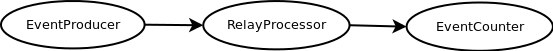
\includegraphics[width=3.0in]{processgraph.png}
	\caption{An example process graph with 3 nodes to count words.}
	\label{processgraph}
\end{figure}

\subsection{Runtime Graph}
When the system is deployed, there can be multiple instances of a particular stage to handle higher loads making the system scalable. Figure \ref{runtimegraph} shows possible runtime graph for process graph shown in Figure \ref{processgraph}. Here each parent process instance sends events to two child process instances. However in this case parent process instance has to pick a child process instance to send the message as well. One way of handling this problem is to pick a random node. Another approach is to send messages with same key to same child process instance. 

\begin{figure}[!t]
        \centering
        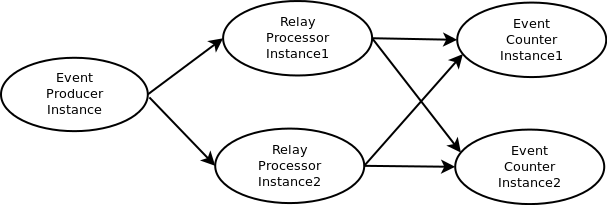
\includegraphics[width=3.0in]{runtimegraph.png}
        \caption{Runtime graph for process graph given in Figure \ref{processgraph}.}
        \label{runtimegraph}
\end{figure}

\subsection{API}
In this section, we explain our API that can be used to define custom events, processes and adapters. We provide clear interfaces to abstract out all the communication complexities from application developers. Table \ref{api} shows details of client interfaces.


\definecolor{dkgreen}{rgb}{0,0.6,0}
\definecolor{gray}{rgb}{0.5,0.5,0.5}
\definecolor{mauve}{rgb}{0.58,0,0.82}

\lstset{frame=tb,
  language=Java,
  aboveskip=3mm,
  belowskip=3mm,
  showstringspaces=false,
  columns=flexible,
  basicstyle={\small\ttfamily},
  numbers=none,
  numberstyle=\tiny\color{gray},
  keywordstyle=\color{blue},
  frame=single,
  breaklines=true,
  breakatwhitespace=true,    
  tabsize=2
}

\begin{table}[ht]
	\centering
	\begin{tabular}{| l | l | l |}
        \hline
        Interface Name &  Method & Parameters \\
        \hline
        Event   & getKey &  \\
        \cline{2-3}
        & serialize &  DataOutput \\
	\cline{2-3}        
        & parse &  DataInput \\
        \hline
        Adapter   & start &  \\
        \cline{2-3}
        & initialize &  Container \\
        \hline
        Processor   & onEvent & Event \\
        \cline{2-3}
        & initialize &  Container \\
        \hline
        \end{tabular}
        \caption{Client API}
        \label{api}
\end{table}


 The \texttt{Event} interface has a method to get the key for a given event. This key is used in sending messages to next processes as described earlier. \texttt{Serialize} method is used to directly convert the event attributes to binary format and \texttt{parse} method is used to directly retrieve event attribute values from binary format. When implementing these methods developers can define attribute serialization order in their \texttt{serialize} method and use the same order during \texttt{parse} method to avoid metadata passing with the binary format. \texttt{Processor} interface contains a method called \texttt{onEvent} which is invoked by the underlying framework when it receives an event to that process. The \texttt{start} method of the \texttt{Adapter} interface is invoked by the framework and that can be used to pull events from external systems once the system starts. During initialization both processes and adapters receive the container that can be used to send events to other processes.
 
 \subsection{Deployment}

As shown in Figure \ref{deployment}, a deployment of the system consists of a manager node and a set of worker nodes. Worker nodes are grouped into clusters so that the application users can specify to which clusters each process needs to get deployed. The Manager node processes applications, deploys them to worker nodes, and initiates the processing by starting the adapters.

\subsection{Application Development}

An application specifies the runtime graph to process a particular event stream. Therefore an application mainly consists of a set of processes, adapters and events and their interactions. Processes, adapters and events can be developed by implementing the respective interfaces as shown above. Then the interactions can be specified using a JSON file. 

\clearpage

\begin{figure}[!t]
        \centering
        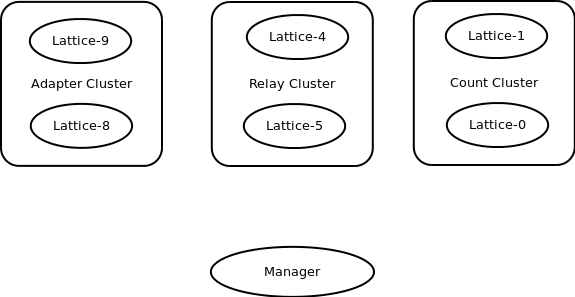
\includegraphics[width=3.0in]{deployment.png}
        \caption{Deployment view of the system with 6 worker nodes into 3 clusters and a Manager node.}
        \label{deployment}
\end{figure}


\lstinputlisting[captionpos=b, label=sampleruntime,caption=Configuration for runtime graph given in Figure \ref{runtimegraph},language=java]{runtimegraph.json}


As shown in Listing \ref{sampleruntime}, the \textit{instances} parameter can be used to specify the required number of instances to be deployed. The \textit{receivers} parameter is used to specify from which process it expects to receive messages and how the sending process should distribute the events among instances. The \textit{key} type indicates that the events with the same key must be received by the same instance. Finally users can deploy the application to manager which processes them and deploys to workers.






 
